\chapter{Perpektivering}
\label{chap:perpektivering}

Perspektivering til byen Graz
Den Østrigske by Graz renoverede i 2011 Sonnenfelsplatz til et shared space område. Sonnenfelsplatz er en central plads som har butikker og restauranter, samt byens universitet campus ligger lige i nærheden %(kilde: http://www.eltis.org/discover/news/shared-space-graz-austria-0 10/12-2015).
 I belastningsperioder har Sonnenfelsplatz i byen Graz i Østrig 15.000 køretøjer, 3.400 fodgængere og 640 cyklister i timen. Dog er det ikke køretøjerne der skaber de fleste trafikbelastninger, men da vejoverfladen er skadet, og infrastrukturen under jorden har haft behov for renovering, blev området lavet om. Herved blev shared space et mål for området, for at skabe en bebolig gade med frit kultur mobilitet, hvor der er plads til alle trafikanttyper. I den anledning er vejskilte og vejafmærkninger bevidst blevet valgt fra, da det vil få de forskellige trafikantgrupper til at integrere sig efter hinanden afhængigt af situationen i området. Dette kan ses tydeligt på vejbanen.
 \begin{figure}[htbp]
   \centering
   \begin{adjustbox}{max width=\textwidth}
     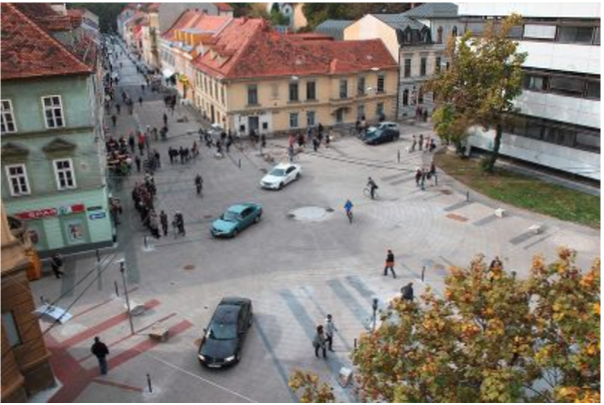
\includegraphics{figures/Billederogfigur/Perspektivering/en_andne_by.png}
  \end{adjustbox}
   \caption{Cykelsti}
    \label{fig:cykelsti}
 \end{figure}
 %(kilde:http://www.stadtentwicklung.graz.at/cms/beitrag/10136328/5030273/ 10/12-2015)
 På Sonnenfelsplatz er der ikke højdeforskel i vejen som adskiller køretøjer fra fodgængere.Trafikanterne deler og respekterer derfor hinanden om pladsen. I midten af pladsen er der lavet en lille rundkørsel.%(kilde:http://www.stadtentwicklung.graz.at/cms/beitrag/10136328/5030273/ 10/12-2015)


I indledningen er Nytorv/Østerågade beskrevet som et samlingspunkt, hvor der på tilsvarende måde færdes mange mennesker og køretøjer. I området er der mange shopping- og cafémuligheder, derudover færdes der mange mennesker i området, som transportere sig med bus og cykel. Ifølge trafiktællingerne der er foretaget i rapporten (se bilag) har Nytorv/Østerågade en års døgns trafik på 394 for biler og 3.826 for cykler på en novemberdag. I interviewet (se bilag) mener flere interviewpersoner, at bilerne og cyklisterne skaber utryghed for fodgængerne, hvilket er årsagen til, at der i rapporten fokuseres på at differentiere trafikantgrupperne. Derved at lave nogle forslag om at etablere en cykelbane i området, hvor cyklisterne kan cykle på deres egen bane, og en bussluse for at udelukke bilerne fra området, hvilket kan ses på de nedenstående billeder.
\begin{figure}[htbp]
  \centering
  \begin{adjustbox}{max width=\textwidth}
    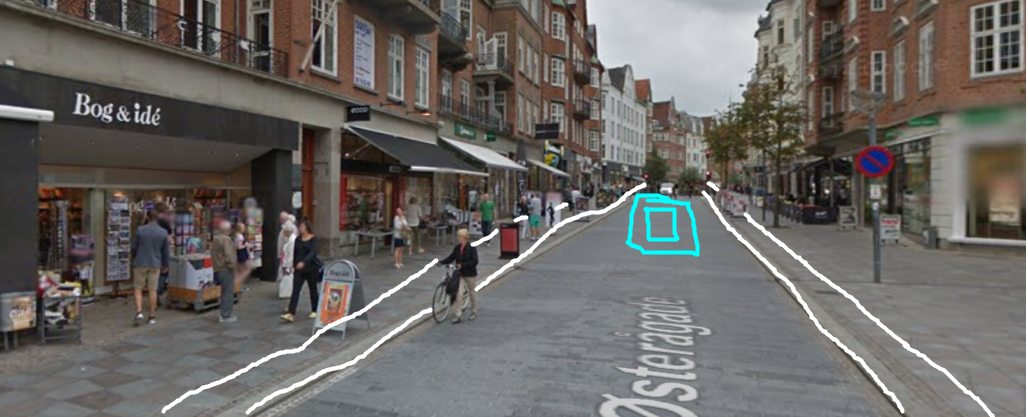
\includegraphics{figures/Billederogfigur/Losningsforslag_cykelsti/Cykelsti_gennem_bogo.png}
 \end{adjustbox}
  \caption{Cykelsti}
   \label{fig:cykelsti}
\end{figure}

\begin{figure}[htbp]
  \centering
  \begin{adjustbox}{max width=\textwidth}
    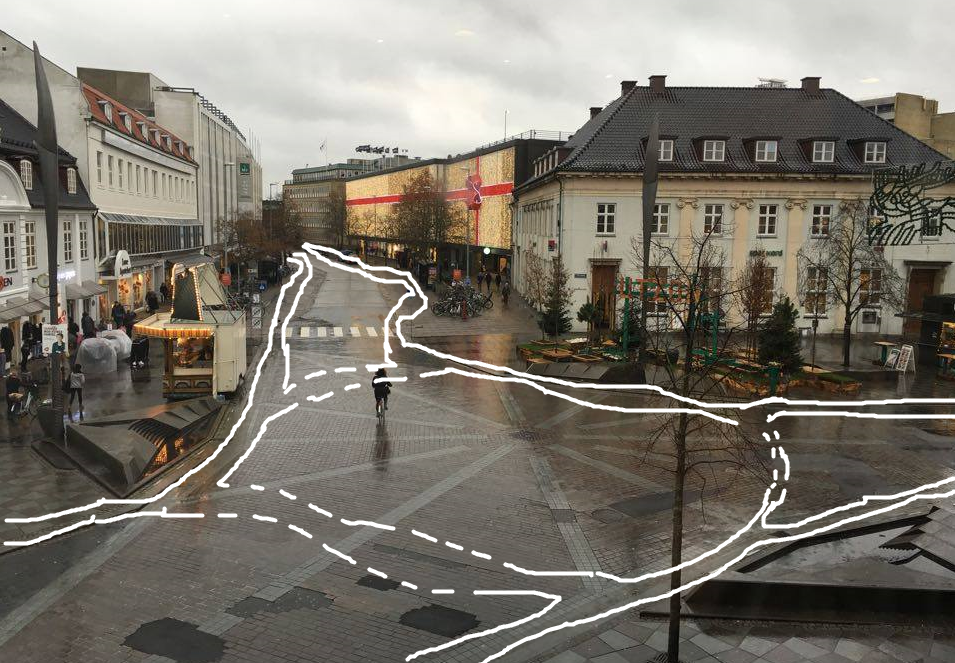
\includegraphics{figures/Billederogfigur/Losningsforslag_cykelsti/cykelsti_ved_knudepunktet.png}
 \end{adjustbox}
  \caption{Cykelsti}
   \label{fig:cykelsti}
\end{figure}

For at kunne afgøre hvad eller hvilke eventuelle løsningsforslag, som løser rapportens undersøgte problemer bedst, er det væsentligt at se på fordele og ulemper ved de forskellige forslag. Ved at etablere en rundkørsel skabes, vil alle trafikantgrupper blive tvunget til at øge deres trafikale fokus, som konsekvens af rundkørslen. Samtidig må det forventes, at deres hastigheder må blive sænket en del. En af ulemperne ved at anlægge en rundkørsel vil på sigt blive en ringere offentlig transport i området, da det kan forsinke bustrafikken at føre dem gennem en rundkørsel på en trafikeret dag. En rundkørsel er særdeles effektiv at bruge som løsningsforslag et sted, hvor der er mange biler, som skal gennem et punkt. Eftersom det største problemfokus på Nytorv ikke er bilerne, men derimod cyklisterne, vil en rundkørsel muligvis gøre mere skade end gavn, hvis en sådan etablering blev en realitet.
Hvis der i stedet rettes fokus på løsningsforslaget med at anlægge en busgrav eller hæve-sænke pullert, er dette forslag, som det forrige, også fokuseret på bil problemet omkring Nytorv. Det ville afhjælpe problemet med de mange uvedkommende biler, der hver eneste dag kører ind i området, trods påbud, som tilsyneladende ikke har den ønskede virkning. En af fordelene bliver hermed, at Nytorv bliver helt fri for uvedkommende biler, og dette vil medvirkende til at skabe et mere forudsigeligt og måske mere trygt trafikmiljø.
Det sidste løsningsforslag beskæftiger sig med en anlægning af cykelbaner i hele området og omkring Nytorv. Fordelene er, at dette er med til at øge fokus på cyklisterne, og det giver et mere klart billede af, hvor cyklerne skal være på vejen. En af de overvejende ulemper er, at en cykelbane vil skabe gnidninger mellem cyklisterne og buspassagererne, når de skal af og på bussen. En cykelbane vil nemlig være etableret langs buslommen, og derved vil buspassagerende være nødsaget til at gå over cykelbanen. Det vil derfor være en nødvendighed, at cyklisterne er opmærksomme og holder tilbage for passagerende.
Da der i forvejen er et forholdsvis smalt fortov nogle steder nede ved Nytorv, bliver det ligeså svært at få plads til de eventuelle cykelbaner. De to første løsningsforslag har fokus på eventuelle bilproblemer, hvorimod det sidste løsningsforslag har til formål at afhjælpe cykelproblemer i trafikken. Eftersom det største trafikale problem nede ved Nytorv er mellem cyklister og fodgængere, er det oplagt at videreudvikle på ideen omkring en cykelbane.
I rapporten har den helt centrale problemstilling været, at undersøge trafikale problemer mellem fodgængere og cyklister ved fodgængerfeltet. Gennem de beregnede TA-værdier og de mange interviews, er der blevet vurderet, at der er et trafikalt problem netop på dette sted mellem cyklisterne og fodgængerne. Bilerne og busserne er gennem de foretagede interviews ikke blevet vurderet til at være et stort problem, og derfor er løsningsforslaget om cykelbanen valgt at blive diskuteret her, som den bedste løsning, for netop denne undersøgelse.
En etablering af en cykelbane vil have til formål at lede cyklisten inde for en afmærket sti, og på den måde fastholde cyklisten inden for afmærkningen Der vil herved blive formået at kontrollere cyklisternes kørebane og opretholde cyklistens fokus i selve kørebanen. Det formodes, at cyklisten vil få øje på en fodgængeren hurtigere, da der ikke er andre trafikanter cyklisten nu skal holde øje med. Det kan muligvis være med til, at man vil kunne observere mange flere tidlige samspil end sene samspil ved fodgængeroverfeltet.. Et sådant formål, ville en etablering af en rundkørsel eller bussluse ikke opfylde. Set i et andet perspektiv, så kan det måske føre til flere kollisioner mellem fodgængere og cyklister, hvis cyklisten ser cykelbanen som sin helt egen bane. Der vil derfor være et dilemma, hvis der ikke bliver taget hensyn til de eventuelle passerende fodgængere eller biler, som svinger ind over cykelbanen. Derfor vil en cykelbane ikke være en endegyldig løsning på konflikterne ved fodgængerfeltet, da det kan tænkes, at der rent faktisk vil kunne opstå flere uheld end før. Men det er klart, at en cykelbane vil kunne guide cyklisterne, og have et bidrag til et mere trygt trafikmiljø på Nytorv/Østerågade området. Dog kan det diskuteres, om det er cyklisten eller fodgængeren, som vil føle sig mere tryg.
